\documentclass[a4paper,12pt]{report}

\usepackage{alltt, fancyvrb, url}
\usepackage{graphicx}
\usepackage[utf8]{inputenc}
\usepackage{float}
\usepackage{hyperref}

\usepackage[italian]{babel}

\usepackage[italian]{cleveref}

\title{Relazione \\``SMOL''}

\author{Ettore Farinelli \\ Marco Galeri \\ Giovanni Paradisi \\ Mounir Samite}
\date{\today}


\begin{document}

\maketitle

\tableofcontents


%------------------------------ANALISI------------------------------
\chapter{Analisi}

%REQUISITI
\section{Requisiti}
Il gruppo si pone come obiettivo quello di realizzare un videogioco 2D arcade con visuale dall’alto di nome "SMOL".
Per arcade si intende una struttura di gioco ripetitiva in cui l'obbiettivo è accumulare più punti possibile.
%

\subsubsection{Requisiti funzionali}
\begin{itemize}
    \item Il software dovrà essere in grado di gestire l'ambiente di gioco durante l'intera durata della partita elaborando le interazioni tra le diverse entità del gioco.
    \item L’obbiettivo del gioco è difendere i campi di ortaggi dalle talpe che invadono la mappa, schiacciandole con un martello. I campi subiranno danni anche in caso 
        il giocatore li attraversi.
    \item Con il progredire dello score la difficoltà di gioco aumenterà, diminuendo il tempo tra la creazione di talpe e modificando la probabilità 
        con cui si generano diversi tipi di talpa.
    \item Durante la partita sarà possibile effetuare diverse operazioni:
    \begin{itemize}
        \item Il giocatore potrà muovere il personaggio, attraverso i tasti direzionali, all’interno della mappa.
        \item Usando il mouse invece, controllerà la direzione del martello che attraverso una pressione prolungata potrà aumentare il raggio di azione.
    \end{itemize}
    \item Il gioco termina quando tutti gli ortaggi risultano distrutti.
\end{itemize}
\subsubsection{Requisiti non funzionali}
\begin{itemize}
    \item Si avrà la possibilità di cambiare l'aspetto grafico scegliendo tra quelli proposti nell'interfaccia del menù.
    \item Il programma sarà in grado di salvare il miglior punteggio in locale.
    \item Il gioco avrà una sezione in cui verrano visualizzate le istruzioni di gioco.
    \item Implementazione di una pagina di game over che permette di tornare al menù senza chiudere l'applicazione e 
        mantenendo lo stesso pacchetto grafico precedentemente utilizzato.
\end{itemize}
%ANALISI E MODELLO DEL DOMINIO
\section{Analisi e modello del dominio}
In SMOL il sofware dovrà essere in grado di controllare le interazioni tra diverse tipologie di entità. 
Tra le entità saranno presenti:
\begin{itemize}
    \item Ortaggi: queste entità fungeranno come vita del giocatore ed a contatto con altre entità perderanno vita
    \item Giocatore: questa entità sarà controllata attraverso la tastiera e permetterà di spostarsi all'interno della mappa.
    \item Martello: questa entità sarà controllata attraverso il mouse che, con una pressione prolungata permetterà di aumentare 
        il proprio raggio di azione, mentre al rilascio, se si troverà a contatto con le talpe, gli toglierà vita.
    \item Talpe: questa entità fungerà da nemico principale del giocatore, spostandosi attraverso la mappa cercherà di mangiare 
        gli ortaggi presenti ed in caso entri in contatto col giocatore gli bloccherà temporaneamente i movimenti.
    \item Muri: impediranno al giocatore di uscire dai confini della mappa di gioco.
\end{itemize}
Il sofware sarà responsabile anche della creazione iniziale degli ortaggi e la generazione delle talpe durante il resto della 
partita attraverso un sistema che incrementerà in base al punteggio corrente del giocatore il numero di talpe generate nel tempo, 
insieme alla probabilità di generare talpe più complicate da abbattere.
Gli elementi costitutivi del dominio sono sintetizzati in %\Cref{img:analysisScheme}.
Per rientrare nel monte ore richiesto non è stato possibile implementare una modalità di multiplayer locale, 
che sarà possibilmente implementata in futuro.

\begin{figure}[H]
\centering{}
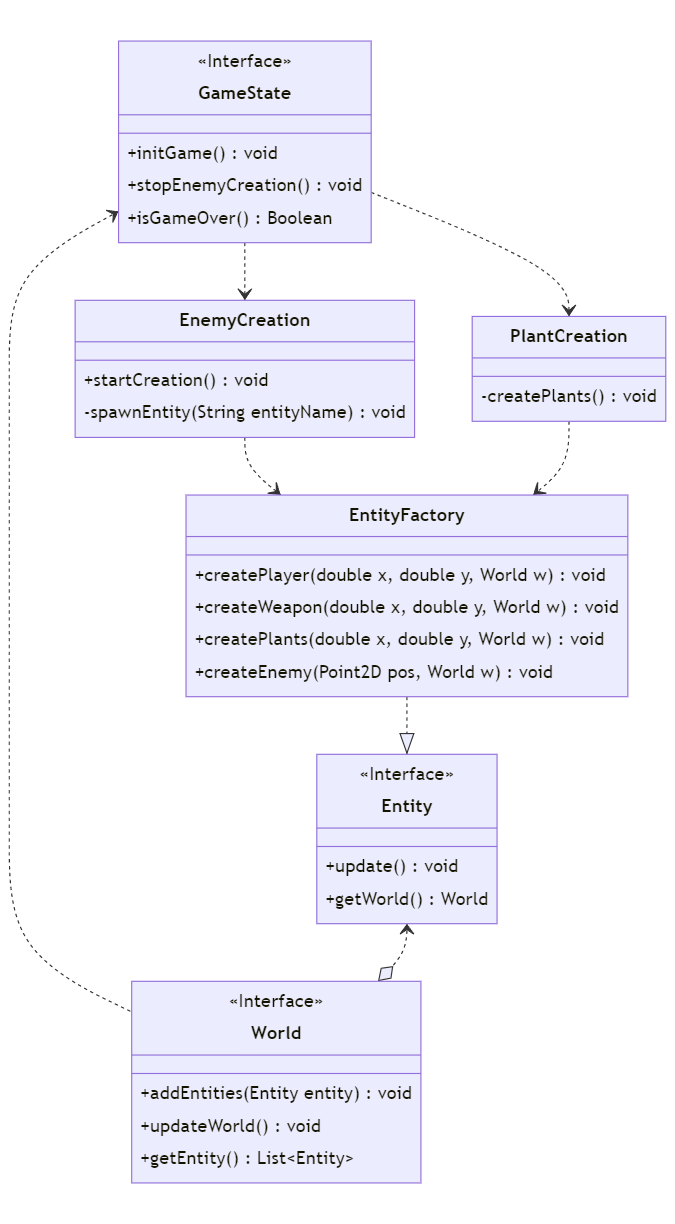
\includegraphics[width=\textwidth,height=0.8\textheight,keepaspectratio]{img/AnalysisUML.png}
\caption{Schema UML dell'analisi del problema, con rappresentate le entità principali ed i rapporti fra loro}
\label{img:analysisScheme}
\end{figure}

%------------------------------DESIGN------------------------------
\chapter{Design}

%ARCHITETTURA
\section{Architettura}
SMOL è stato progettato seguendo lo schema architetturale del \textsc{MVC} applicando però la struttura del \textsc{ECS} per la gestione 
delle entità.

\begin{figure}[h]
\centering{}
%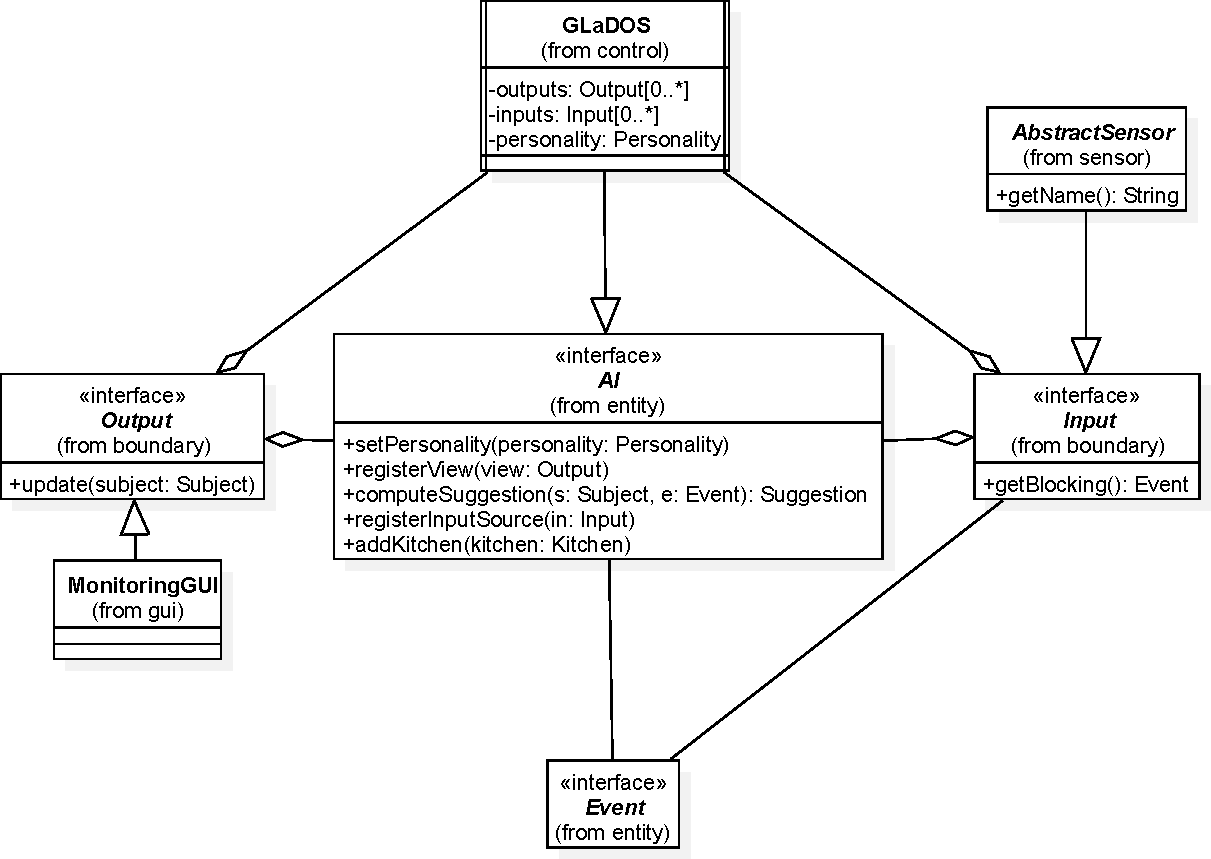
\includegraphics[width=\textwidth]{img/arch}
\caption{Schema UML raffigurante l'architettura di SMOL.}
\label{img:goodarch}
\end{figure}

%DESIGN DETTAGLIATO
\section{Design dettagliato}

\subsection*{Ettore Farinelli}
\subsubsection{Implementazione degli input del giocatore}
\begin{figure}[H]
\centering{}
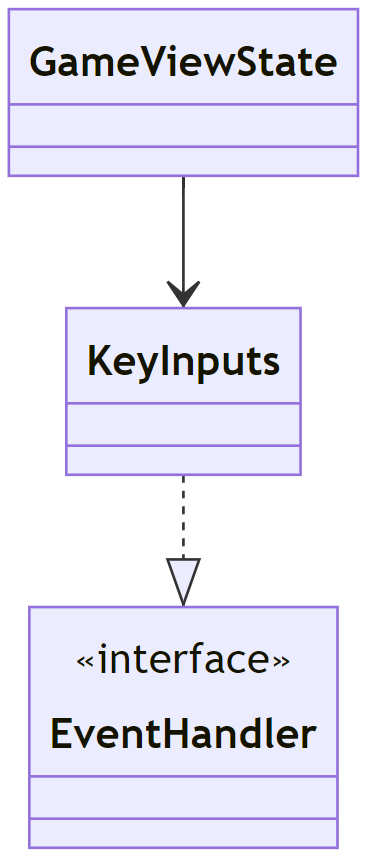
\includegraphics[scale = 0.5]{img/KeyInputsUML.PNG}
\caption{Schema UML rappresentante il ricevimento degli input della classe \emph{KeyInputs}.}
\end{figure}
\paragraph{Problema}
    Un input inserito da tastiera deve essere elaborato e immagazzinato cosi da permettere al player di muoversi.
\paragraph{Soluzione}
    Ogni input inserito da tastiera viene ricevuto e passato alla classe \emph{KeyInputs} che lo filtra e in base al tipo  
    inserisce una \emph{Direction} all'interno di una coda che verrà successivamente svuotata un elemento alla volta 
    dall'\emph{InputComponent} (in questo caso dal \emph{PlayerInputComponent}) ricevendo così le direzioni che verranno 
    applicate all'entità stessa permettendole di muoversi nella mappa di gioco, Come da figura\ref{img:PlayerMovement}.
\begin{figure}[H]
\centering{}
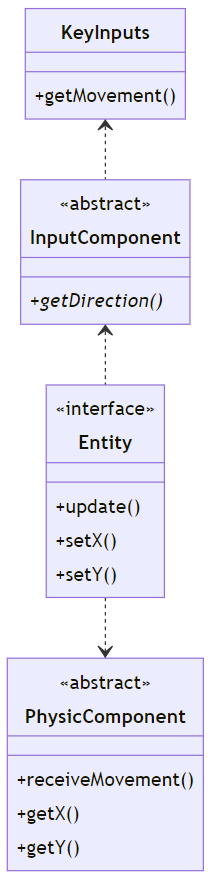
\includegraphics[scale = 0.5]{img/PlayerMovement.PNG}
\caption{Schema UML che rappresenta in che modo un input venga elaborato e ricevuto da un entità.}
\label{img:PlayerMovement}
\end{figure}

\subsubsection{Gestione del martello}
\begin{figure}[H]
\centering{}
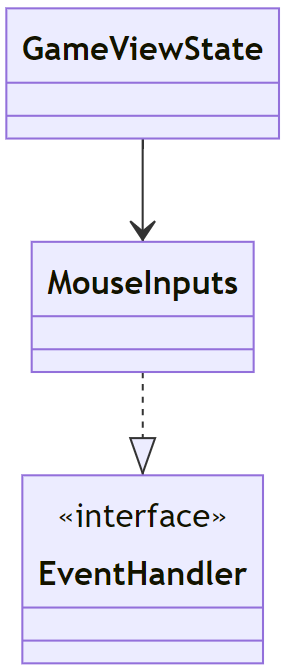
\includegraphics[scale = 0.5]{img/MouseInputsUML.PNG}
\caption{Schema UML rappresentante il ricevimento degli input della classe \emph{MouseInputs}.}
\end{figure}
\paragraph{Problema}
    Il martello dovrà avere una posizione risultante distante dal giocatore di una misura uguale al raggio della circonferenza 
    di diamentro \textsc{weaponRange} e in una posizione presente nella retta tracciata dal centro del giocatore al cursore del mouse.
    Inoltre quando il martello viene rilasciato dovrà bloccare gli input per permettere al player (virtualmente) di colpire con 
    il martello la talpa su cui il bersaglio si trova.
\paragraph{Soluzione}
    Come per il problema degli input da tastiera, quelli da mouse vengono ricevuti e elaborati in maniera simile con una differenza
    sostanziale. Infatti, \emph{MouseInputs} salva direttamente la posizione del cursore
    quando viene mosso o rilasciato, che viene quindi ricevuta dall'\emph{InputComponent} e poi elaborata nel \emph{PhysicComponent} 
    dove vengono quindi fatti tutti i calcoli \footnote{\url{https://github.com/TheDarkRuler/OOP22-SMOL/blob/757228125cb2531fccca35b35f7645ceba9d5ae9/src/main/java/it/unibo/smol/model/impl/physicscomponent/WeaponPhysicsComponent.java#L46-L51}} 
    per trovare la effettiva posizione in cui il martello colpirà al rilascio\ref{img:MouseInputs}. Sempre al rilascio del tasto sinistro del mouse, 
    per bloccare gli input da tastiera e da mouse inizialmente ho pensato di utilizzare dei metodi, e quindi campi, statici 
    accessibili sia da \emph{MouseInputs} che da \emph{KeyInputs}, infine poi, a seguito di diverse migliorie 
    ho optato per includere un campo di tipo \emph{KeyInputs} all'interno di \emph{MouseInputs} così da poter notificare il blocco 
    degli input da una classe all'altra.
\begin{figure}[H]
\centering{}
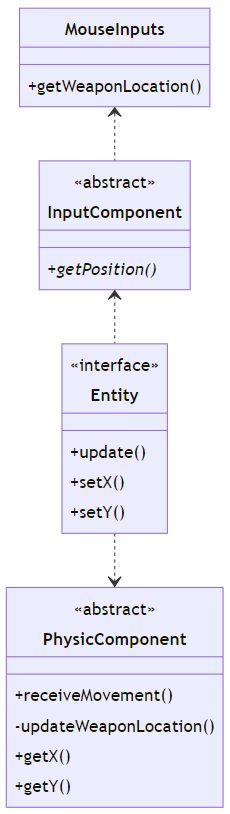
\includegraphics[scale = 0.5]{img/MouseInputs.PNG}
\caption{Schema UML che rappresenta in che modo un input venga elaborato e ricevuto da un entità.}
\label{img:MouseInputs}
\end{figure}

\subsubsection{Creazione AI talpe}
\begin{figure}[H]
\centering{}
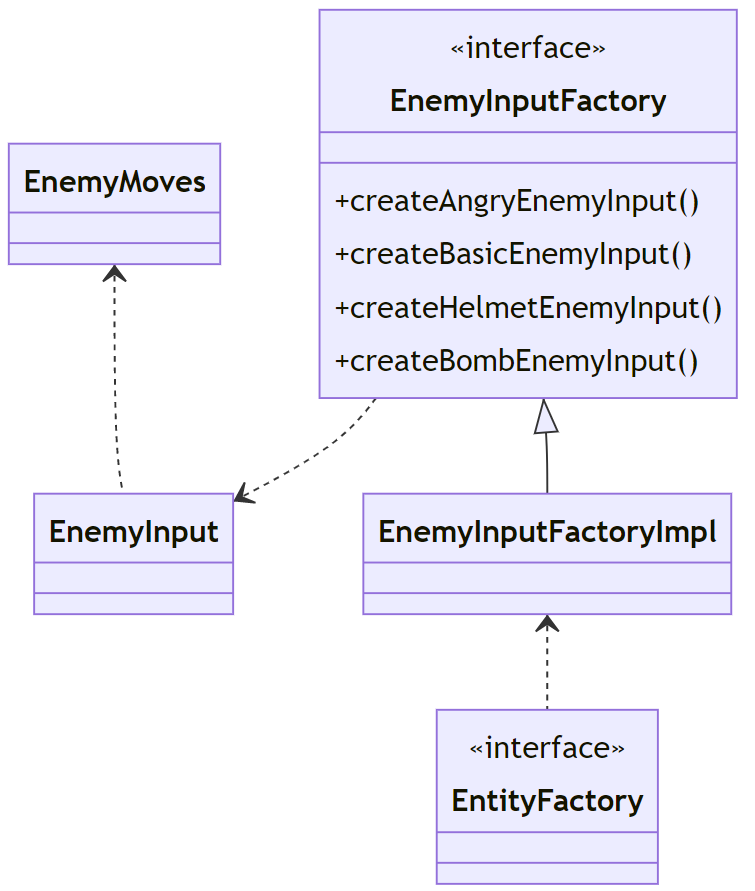
\includegraphics[scale = 0.5]{img/EnemyInputs.PNG}
\caption{Schema UML rappresentante lo schema di ereditarietà della classe EnemyInput.}
\end{figure}

\paragraph{Problema}
    Creare un intelligenza artificiale che scelga una posizione, dove non siano presenti altre entità al momento, in modo 
    pseudo-casuale e che sia adattabile a 4 diversi tipi di entità. Inoltre essa deve effettivamente muoversi nella mappa 
    in maniera uniforme.
\paragraph{Soluzione}
    Per creare un tipo di intelligenza artificiale che stimoli il più possibile il giocatore con movimenti casuali e variabili 
    ho deciso di dare alle entità nemiche un tipo di movimento che divida la mappa di gioco in quattro quadranti e casualmente 
    scelga uno dei quadranti dove, ancora una volta casualmente scelga una posizione in esso non occupata da altre entità, 
    così che la posizione futura di una talpa sia prevedibile il meno possibile. Per il problema del movimento uniforme 
    della talpa ho deciso di effetuare dei calcoli per trovare il giusto passo che essa deve fare per muoversi 
    nell'asse delle ascisse e in quello delle ordinate \footnote{\url{https://github.com/TheDarkRuler/OOP22-SMOL/blob/3d89bb7d9ef1c36e091a01eed47fa5c9fcbe6486/src/main/java/it/unibo/smol/controller/input/EnemyMoves.java#L68-L70}}
    che le viene applicato dall'\emph{InputComponent} attraverso l'\emph{Entity} permettendole di modificare a mano a mano la sua posizione.
    Infine per la creazione degli input inizialmente ho creato una classe che veniva estesa da altre classi che definivano 
    ognuno un tipo di talpa, in seguito rianalizzando il codice, ho notato di poter attuare il \emph{Factory Pattern}, dando così 
    la possibilità di creare i 4 tipi di input attraverso una sola classe rendendo più comprensibile e intuitiva la creazione 
    di input nella \emph{EntityFactory}, inoltre facilitando la possibile implementazione futura di un nuvo tipo di nemico.

\subsubsection{Gestione delle collisioni}
\begin{figure}[H]
\centering{}
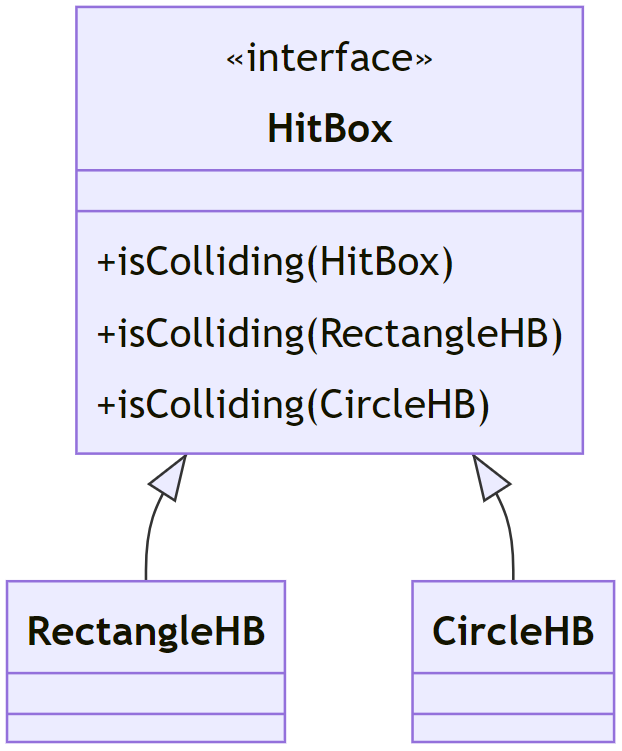
\includegraphics[scale = 0.5]{img/HitBox.PNG}
\caption{Schema UML rappresentante l'utilizzo del \emph{Visitor Pattern} per il controllo delle collisioni tra diverse forme.}
\end{figure}

\paragraph{Problema}
    L'oggetto su cui viene chiamato il metodo \textsc{isColliding} ha bisogno di conoscere di che tipo di HitBox è il parametro 
    che gli viene passato.
\paragraph{Soluzione}
    Per la soluzione di questo problema ho deciso di implementare il pattern \emph{Visitor} permettendo così di facilitare una possibile 
    implementazione futura di una nuova HitBox di forma diversa, in quanto il controllo della collisione viene affidato all'oggetto 
    che viene passato alla chiamata del metodo, evitando cosi controlli manuali riguardanti lo stato del parametro.
\subsection*{Marco Galeri}

\subsubsection{Gestione delle Entità}

\begin{figure}[H]
\centering
    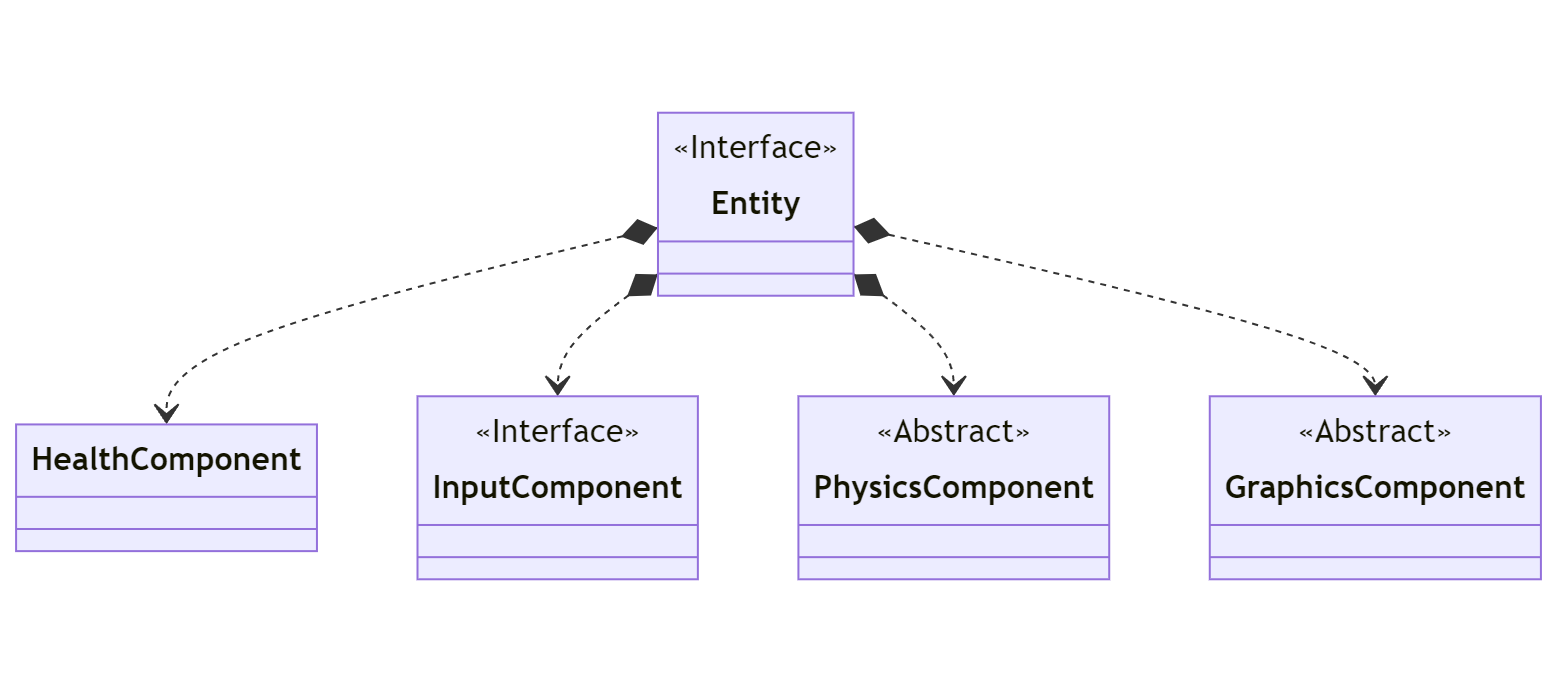
\includegraphics[width=\textwidth,height=2\textheight,keepaspectratio]{img/EntityUML.png}
    \caption{Rappresentazione UML di una entità e i suoi componenti}
\end{figure}

\paragraph{Problema}
    L'interfaccia \textsc{Entity} deve implementare numerosi comportamenti diversi, l'uso dell'ereditarietà porterebbe alla creazione di molteplici sottoclassi ed a possibili problemi di eredità multipla aumentando la complessità del codice. Inoltre la classe \textsc{Entity} incapsula diversi aspetti del gioco violando il \textit{Single Responsability Principle}.

\paragraph{Soluzione}
    Adottando l'\textit{Entity Component System}, ampiamente usato nell'ambito di Game Development, si ha una scissione dei vari aspetti di gioco in \textsc{components}. L'unione dei \textsc{components} quindi definisce il comportamento finale di ogni Entità. Con questo design che favorisce la composizione al posto dell'ereditarietà si ha un aumento di flessibilità del codice che viene suddiviso in classi più corte e meno complicate. Inoltre i componenti sono altamente riusabili rendendo plausibile la creazione di diverse tipologie di entità e lasciando libera la possibilità di aggiunte future.

\subsubsection{Creazione delle Entità}

\begin{figure}[H]
\centering{}
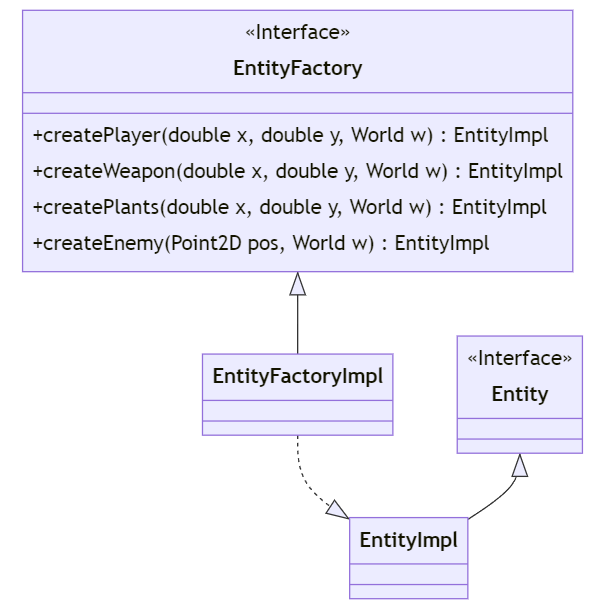
\includegraphics[width=0.75\textwidth,keepaspectratio]{img/EntityFactoryUML.png}
\caption{Rappresentazione UML della creazione di una entità attraverso l'utilizzo del Factory method}
\end{figure}

\paragraph{Problema}
    Date le molteplici tipologie di componenti che una Entità può avere, la creazione di un'Entità direttamente all'interno del mondo è possibile ma poco flessibile e funzionale. 
    
\paragraph{Soluzione}
    Impiegando il \textit{Factory design pattern},  la creazione dell'entità viene esternalizzata in una classe. Con questa classe, \textsc{EntityFactory}, si possono creare dei set di componenti predefiniti da usare per istanziare ogni tipo di entità. Attraverso questo metodo si diminuisce notevolmente la duplicazione di codice, inoltre si rimuove la responsabilità di creazione delle entità dalla classe chiamante. 

\subsubsection{Gestione del movimento e risoluzione delle collisioni tra Entità}

\begin{figure}[H]
\centering{}
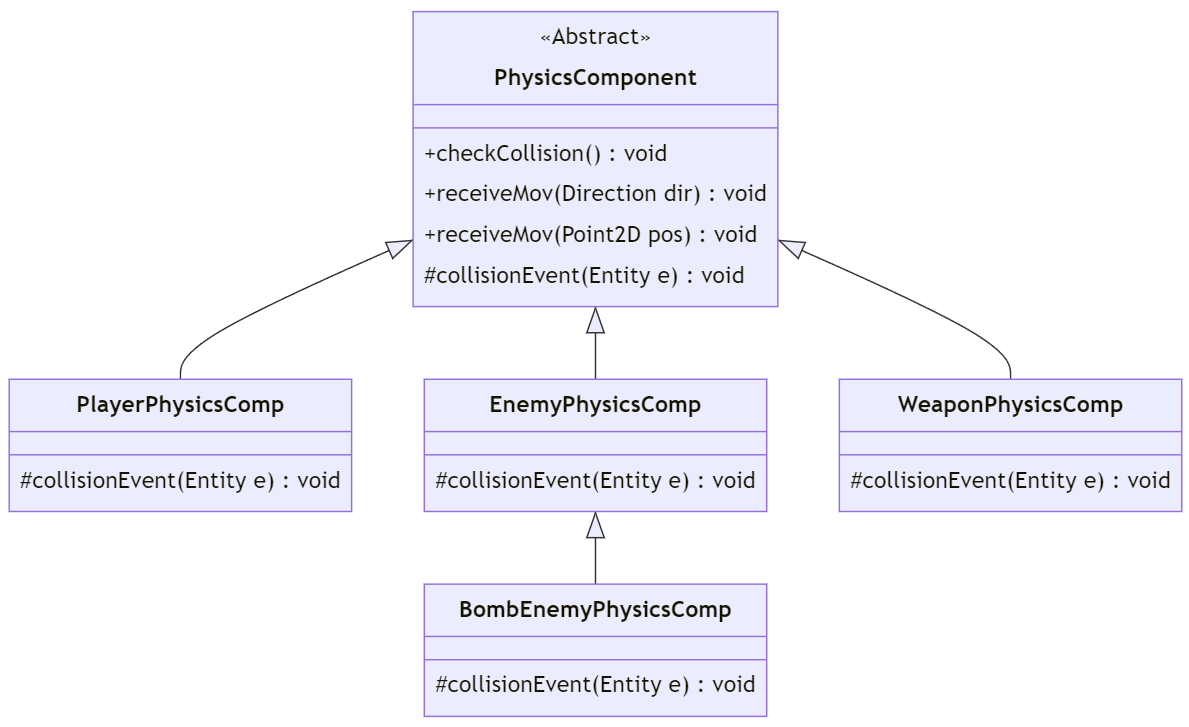
\includegraphics[width=1\textwidth,keepaspectratio]{img/PhysicsComponentUML.png}
\caption{Rappresentazione UML delle diverse interazioni tra Entità}
\end{figure}

\paragraph{Problema}
\begin{itemize}
    \item Entità diverse ricevono comandi di movimento differenti rendendo complicato creare una interfaccia generale che gestisca la fisica delle entità.
    \item Le collisioni devono produrre eventi differenti in base alle tipologie di Entità che stanno collidendo.
\end{itemize}

\paragraph{Soluzione}
    Utilizzando un \textit{Template method pattern} si ha la possibilità di definire una struttura generale della classe, lasciando alle sottoclassi la scelta di dettagli specifici. Questo riduce drasticamente la duplicazione di codice in quanto i metodi template \texttt{checkCollision()} e \texttt{receiveMovement()} vengono scritti unicamente nella classe madre. Inoltre tramite l'overload del metodo \texttt{receiveMovement()} viene generalizzata anche la funzione di movimento.
    
\subsubsection{Gestione di input multipli}

\begin{figure}[H]
\centering{}
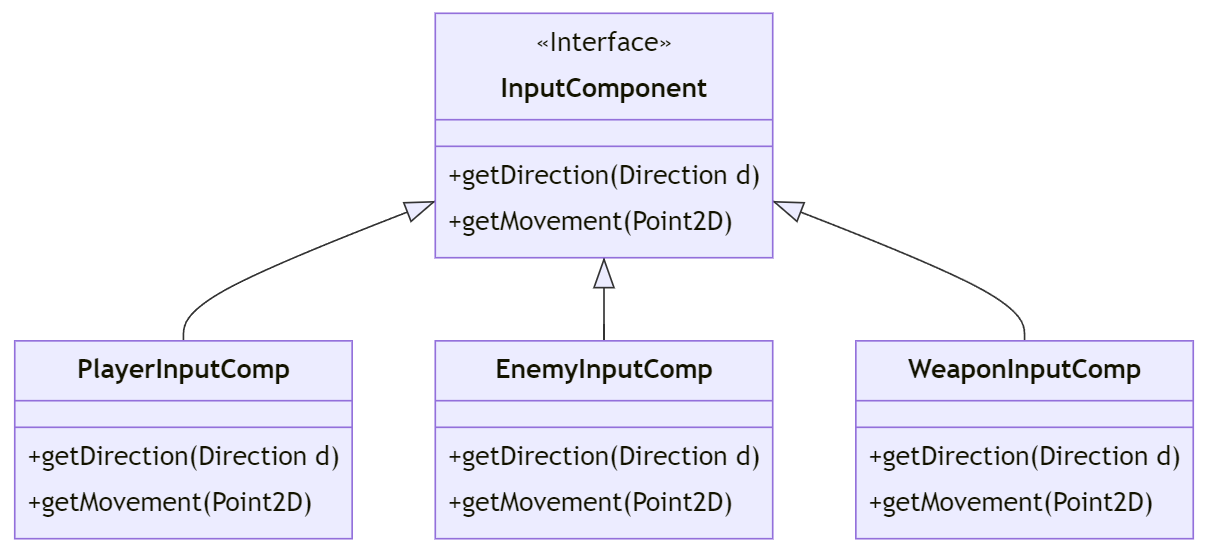
\includegraphics[width=\textwidth,keepaspectratio]{img/InputComponentUML.png}
\caption{Rappresentazione UML della gestione degli InputComponent}
\end{figure}

\paragraph{Problema}
\begin{itemize}
    \item L'utilizzo di diverse implementazioni di input richiede la presenza di una interfaccia generale che li gestisca
    \item L'implementazione di nuove periferiche di gioco può risultare scomodo e macchinoso
\end{itemize}
\paragraph{Soluzione}
L'utilizzo di uno \textit{Strategy pattern} consente di isolare le diverse implementazioni di \textsc{InputComponent} randendole facilmente intercambiali e propense ad aggiunte future.
    
\subsection*{Giovanni Paradisi}
roba di Giovanni
\subsection*{Mounir Samite}
\subsubsection*{Gestione delle finestre}
\begin{figure}[h]
\centering{}
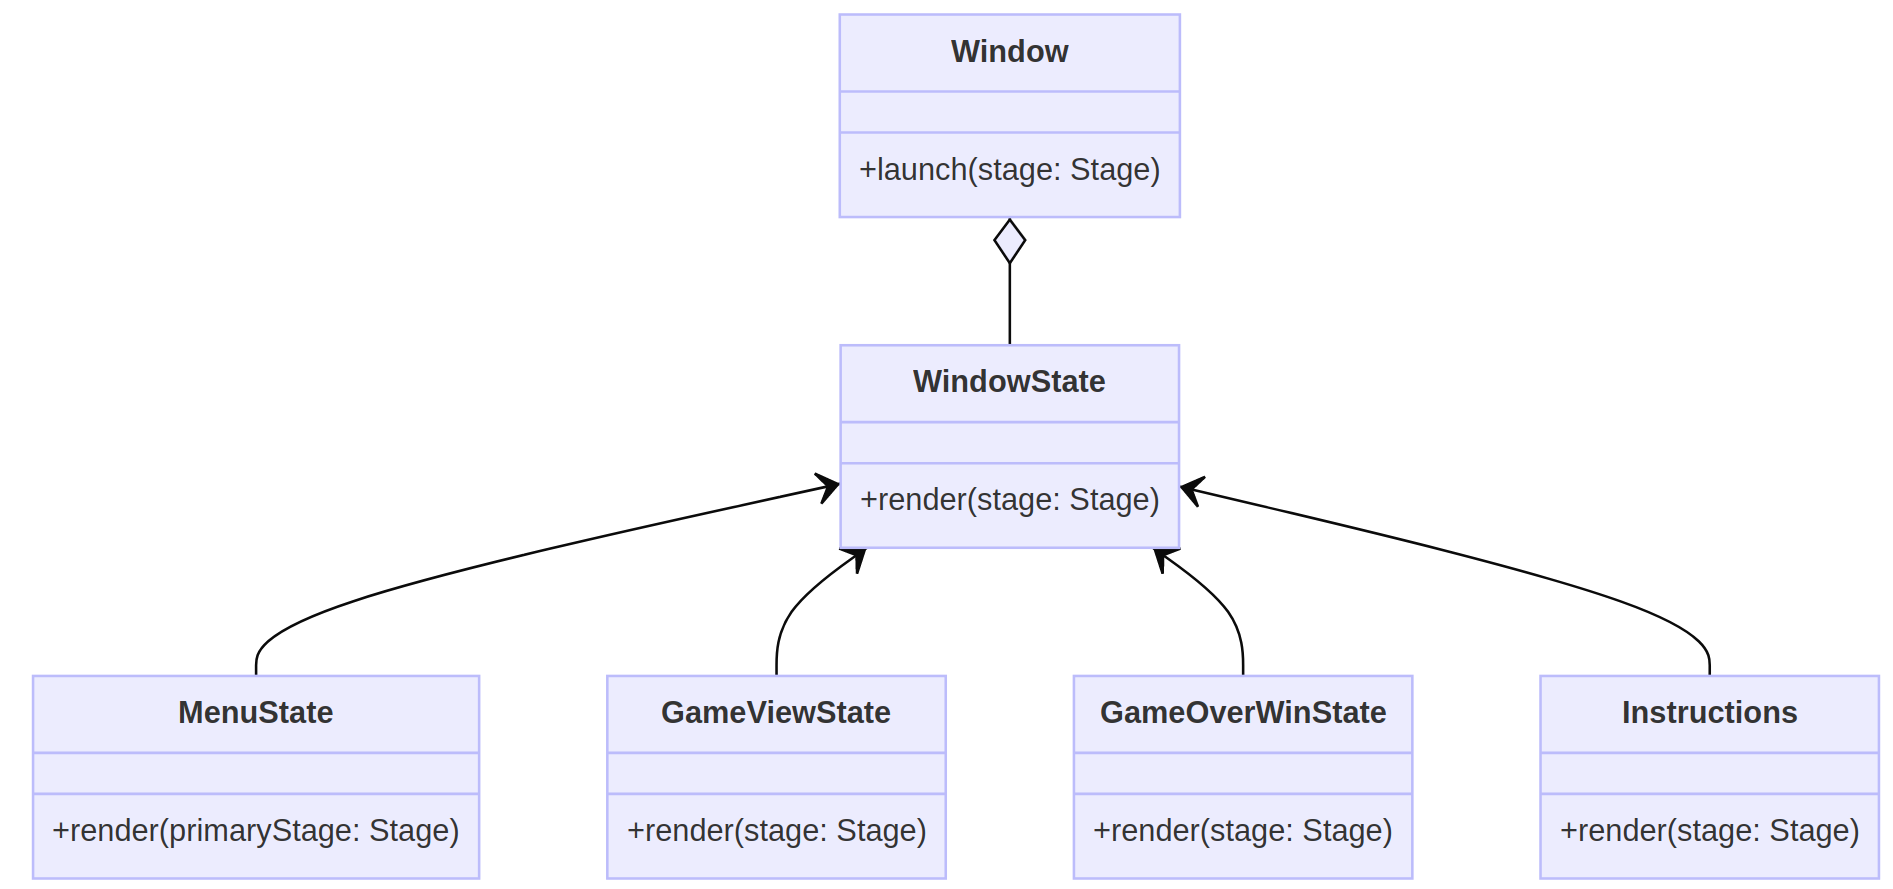
\includegraphics[width=1\textwidth]{img/WindowManagement.png}
\caption{Schema UML della gestione delle finestre del gioco usando lo state pattern}
\end{figure}
\paragraph*{Problema} gestire le finestre del software, favorendo la modularità.
\paragraph*{Soluzione} Il pattern State è utile per gestire le finestre in un videogioco con JavaFX poiché 
consente di gestire lo stato di una finestra in modo dinamico e di cambiare facilmente lo stato della finestra a seconda delle esigenze 
dell'applicazione. In un videogioco, ad esempio, ci possono essere diverse finestre con diverse funzionalità, come la finestra di gioco, 
la finestra del menu, la finestra del game over e così via.
\\
Utilizzando il pattern State, si può creare una classe per ogni stato possibile della finestra e gestire i comportamenti specifici 
di ogni stato all'interno della sua classe. In questo modo, si può garantire che la finestra si comporti
 in modo corretto a seconda dello stato in cui si trova.
 \\
 In questo modo, è possibile cambiare lo stato della finestra in modo dinamico a seconda delle azioni dell'utente o del gioco stesso,
  senza dover scrivere codice ripetitivo o complicato. 
 Inoltre, questo approccio favorisce la modularità del codice, rendendolo più facile da mantenere e riutilizzare.


%------------------------------SVILUPPO------------------------------
\chapter{Sviluppo}

%TESTING
\section{Testing automatizzato}

Per effettuare i test abbiamo utilizzato la libreria JUnit 5.9.1
\\I test automatizzati che abbiamo effettuato sono:
\begin{itemize}
    \item \textbf{HitBoxTest}: in questa classe si testano le collisioni tra le diverse forme presenti nel gioco assicurandosi il corretto funzionamento.
    
    \item \textbf{EnemyInputTest}: in questa classe si verifica se, alla creazione di un EnemyInput, le variabili vengono correttamente 
        inizializzate e se \emph{EnemyTimesSpawn} incrementa.
    
    \item \textbf{KeyInputsTest}: in questa classe si controlla che, quando viene premuto o rilasciato un tasto, vengono correttamente 
        inserite le \emph{Direction} nella coda assicurandosi invece che non vengano aggiunti elementi in caso il player risulti bloccato. 
    
    \item \textbf{MouseInputsTest}: in questa classe si controlla che tutte le variabili della classe \emph{MouseInputs}  
        assumono correttamente determinati valori quando necessario.
    
    \item \textbf{GameStateTest}: in questa classe si testa il sistema di punteggio, che dovrà aumentare e diminuire come previsto senza mai scendere sotto lo zero. Inoltre verrano testate l'inizializzazione del gioco, assicurandosi della creazione dei corretti elementi e la condizione di Game Over.
    
    \item \textbf{EntityTest}: in questa classe si controlla la corretta creazione delle entità controllando la presenza di componenti specifici per ogni tipologia.
    
    \item \textbf{HealthTest}: in questa classe vengono testate le funzionalità di aumento o perdita di vita e la condizione di morte delle Entità assicurandosi il corretto funzionamento.
    
    \item \textbf{PhysicsTest}: in questa classe vengono testate le interazioni tra le diverse entità assicurandosi il corretto funzionamento degli eventi scatenati da esse.
    
    \item \textbf{WorldTest}: in questa classe si controlla la corretta inizializzazione del mondo e si testano le funzioni di manipolazione della lista di Entità assicurandosi il corretto funzionamento.
\end{itemize}

%METODOLOGIA_DI_LAVORO
\section{Metodologia di lavoro}

Siamo partiti inizialmente con un'attenta analisi del dominio del gioco e di cosa potesse essere aggiunto, cercando di rendere il gioco adeguatamente estendibile.
Dunque è stato fatto un UML generale per avere in mente il funzionamento del gioco e sono state definite tutte le principali interfacce.
Invece per quanto riguarda il workflow è stata adottata la metodologia di DVCS semplice, spiegata a lezione, con pull e push.

\subsection*{Ettore Farinelli}
Mi sono occupato di:
\begin{itemize}
    \item Gestione delle collisioni (\textbf{package smol.common, smol.common.hitbox}).
    \item \emph{EnemyInput} e \emph{EnemyInputFactory} (\textbf{package smol.controller.api}).
    \item Gestione degli input e movimento talpe (\textbf{package smol.controller.input}).
    \item \emph{plantsCreation} (\textbf{package smol.model.impl}).
    \item \emph{GraphicsDraw} e \emph{GameViewState} (\textbf{package smol.view.impl}).
\end{itemize}

Ho inoltre contribuito a:
\begin{itemize}
    \item \emph{EnemyCreation} (\textbf{package smol.model.impl}).
    \item \emph{PhysicComponent} implementando il receiveMovement del \emph{WeaponPhysicsComponent} (\textbf{package smol.model}).
    \item \emph{LoadImgs} aggiungendo la mappa per la scelta del pacchetto di skin (\textbf{package smol.view}).
\end{itemize}
\subsection*{Marco Galeri}

Mi sono occupato di:
\begin{itemize}
    \item \emph{GameEngine} e \emph{GameLoop} (\textbf{package smol.core})
    \item \emph{Entity} ed \emph{EntityFactory} (\textbf{package smol.model})
    \item \emph{PhysicsComponent} e le sue sottoclassi (\textbf{package smol.model})
    \item \emph{HealthComponent} (\textbf{package smol.model.impl})
    \item \emph{InputComponent} (\textbf{package smol.controller})
    \item rendere la grafica proporzionale allo schermo (\textbf{package smol.view.GameMap})
\end{itemize}

Ho inoltre contribuito a:
\begin{itemize}
    \item \emph{GameViewState} Aggiungendo il punteggio (package smol.view)
\end{itemize}

\subsection*{Giovanni Paradisi}

Mi sono occupato di:
\begin{itemize}
    \item \emph{GameState} (\textbf{package smol.controller})
    \item \emph{GraphicComponent}, le sue sottoclassi e la classe \emph{LoadImgs} (\textbf{package smol.view})
    \item Implementazione delle istruzioni di gioco nella classe \emph{InstructionsState} (\textbf{package smol.view})
    \item \emph{EnemyCreation} (\textbf{package smol.model})
    \item Salvataggio in locale del record \emph{ScoreLocalStorage} (\textbf{package smol.model})
\end{itemize}

Ho inoltre contribuito a:
\begin{itemize}
    \item \emph{GameViewState} aggiungendo il record (package smol.view)
\end{itemize}

\subsection*{Mounir Samite}
Mi sono occupato di:
\begin{itemize}
    \item Progettazione dell'utilizzo delle finestre con \emph{Window} e \emph{WindowState} con cui verranno renderizzate tutti i tipi di finestre come Menu, Gioco e Game Over (\textbf{package it.unibo.smol.view});
    \item Implementazione del Menu di gioco nella classe \emph{MenuState} (\textbf{package it.unibo.smol.view});
    \item Implementazione del GameOver (fine gioco) nella classe \emph{GameOverWinState} (\textbf{package it.unibo.smol.view});
    \item Progettazione del Mondo di gioco ovvero del contenitore di tutte le entità, degli input e dello score andando a gestire alcune loro funzionalità in \emph{WorldImpl} (\textbf{package it.unibo.smol.model});
    \item Progettazione della barra della vita del player in \emph{HealthBarTankImpl} (\textbf{package it.unibo.smol.view}).
\end{itemize}
Ho inoltre contribuito a:
\begin{itemize}
    \item \emph{PlayerInputComponent} (\textbf{package it.unibo.smol.controller});
    \item \emph{WeaponInputComponent} (\textbf{package it.unibo.smol.controller});
    \item \emph{GameViewState} andando a gestire la barra della vita anche li (\textbf{package it.unibo.smol.view});
    \item \emph{GameEngine} aggiungendo le skins (che in questo caso sono intese come diversi tipi di grafica) al gioco: vettoriale e pixelata per ora (\textbf{package it.unibo.smol.core}) 
\end{itemize}

%NOTE_DI_SVILUPPO
\section{Note di sviluppo}

\subsection*{Ettore Farinelli}
\subsubsection{Utilizzo di stream}
\begin{itemize}
    \item Scelta, di una talpa, della pianta su cui andare: 
        \url{https://github.com/TheDarkRuler/OOP22-SMOL/blob/7c96b119ea8cc75403c5656491ac352c0466de73/src/main/java/it/unibo/smol/controller/api/EnemyInput.java#L197-L217}
\end{itemize}

\subsubsection{Utilizzo di Lambda Expressions}
\begin{itemize}
    \item \url{https://github.com/TheDarkRuler/OOP22-SMOL/blob/7c96b119ea8cc75403c5656491ac352c0466de73/src/main/java/it/unibo/smol/view/impl/GameViewState.java#L147}
\end{itemize}
\subsection*{Marco Galeri}

Il GameLoop è stato realizzato ispirandosi al capitolo "GameLoop" presente in \emph{Game Programming Patterns}\footnote{\url{https://gameprogrammingpatterns.com/}} di Robert Nystrom.

\subsubsection{Utilizzo di Stream}
\begin{itemize}
    \item Controllo delle collisioni: \url{https://github.com/TheDarkRuler/OOP22-SMOL/blob/757228125cb2531fccca35b35f7645ceba9d5ae9/src/main/java/it/unibo/smol/model/api/PhysicsComponent.java#L34-49}

\end{itemize}

\subsection*{Giovanni Paradisi}

\subsubsection{Utilizzo di Stream}
\begin{itemize}
    \item SpawnEnemies: \url{https://github.com/TheDarkRuler/OOP22-SMOL/blob/7c96b119ea8cc75403c5656491ac352c0466de73/src/main/java/it/unibo/smol/model/impl/EnemyCreation.java#L110-L116}
\end{itemize}

\subsubsection*{Utilizzo di JavaFX}
\begin{itemize}
    \item Utilizzo di FXML nelle \emph{Instructions}: \url{https://github.com/TheDarkRuler/OOP22-SMOL/blob/master/src/main/java/it/unibo/smol/view/impl/InstructionsState.java#L61}
\end{itemize}

\subsection*{Mounir Samite}
\subsubsection*{Utilizzo di Stream per gestione delle entità}
\begin{itemize}
    \item Prendere le talpe dalla lista di entità: \url{https://github.com/TheDarkRuler/OOP22-SMOL/blob/dac2df26a7ed60c955c6ea339cb908958a450955/src/main/java/it/unibo/smol/model/impl/WorldImpl.java#L49-L55}
    \item Prendere le piante dalla lista di entità: \url{https://github.com/TheDarkRuler/OOP22-SMOL/blob/dac2df26a7ed60c955c6ea339cb908958a450955/src/main/java/it/unibo/smol/model/impl/WorldImpl.java#L63-L69}
    \item Rileva il player dalla lista di entità: \url{https://github.com/TheDarkRuler/OOP22-SMOL/blob/dac2df26a7ed60c955c6ea339cb908958a450955/src/main/java/it/unibo/smol/model/impl/WorldImpl.java#L56-L62}
\end{itemize}
\subsubsection*{Utilizzo di JavaFX}
\begin{itemize}
    \item Utilizzo di javaFX senza FXML per la gestione della health bar in \emph{GameViewState}: \url{https://github.com/TheDarkRuler/OOP22-SMOL/blob/1a17f10567507032ae1308ff28c6147b7e08646a/src/main/java/it/unibo/smol/view/impl/GameViewState.java#L164-L201}
    \item Utilizzo di FXML nel \emph{MenuState} e nel \emph{GameOverWinState}: \url{https://github.com/TheDarkRuler/OOP22-SMOL/blob/1a17f10567507032ae1308ff28c6147b7e08646a/src/main/java/it/unibo/smol/view/impl/MenuState.java#L80}
    \item Utilizzo basilare di CSS con FXML: \url{https://github.com/TheDarkRuler/OOP22-SMOL/blob/1a17f10567507032ae1308ff28c6147b7e08646a/src/main/resources/css/Menu.css}
\end{itemize}

\subsection*{Utilizzo di Lambda Expressions}
\begin{itemize}
    \item \url{https://github.com/TheDarkRuler/OOP22-SMOL/blob/1a17f10567507032ae1308ff28c6147b7e08646a/src/main/java/it/unibo/smol/view/impl/HealthBarTankImpl.java#L71-L76}
    \item \url{https://github.com/TheDarkRuler/OOP22-SMOL/blob/1a17f10567507032ae1308ff28c6147b7e08646a/src/main/java/it/unibo/smol/model/impl/WorldImpl.java#L132-L136}
\end{itemize}

%------------------------------COMMENTI_FINALI------------------------------
\chapter{Commenti finali}

%AUTOVALUTAZIONE_E_LAVORI_FUTURI
\section{Autovalutazione e lavori futuri}
\subsection*{Ettore Farinelli}
Sono deicsamente soddisfatto del risultato ottenuto dal nostro lavor
\subsection*{Marco Galeri}
Ho apprezzato molto la possibilità di realizzare un simile progetto, essendo la prima volta in cui ci cimentavamo in un progetto di questa portata le difficoltà non sono mancate ma siamo riusciti comunque a consegnare un programma di cui mi ritengo abbastanza soddisfatto.
 Questo progetto mi ha fatto realizzare quanto non sia scontato un buon lavoro di squadra.
 Comunque nonostante una partenza poco cooperativa nella fase di analisi e progettazione siamo riusciti a collaborare in modo efficiente nelle fasi successive.
 Detto ciò penso che il progetto abbia del potenziale e spero di riuscire a migliorare in futuro.
\subsection*{Giovanni Paradisi}
roba di Giovanni
\subsection*{Mounir Samite}
Inizierò dicendo che ho apprezzato molto il nostro lavoro di squadra su questo progetto. Tutti abbiamo dimostrato un grande impegno e dedizione nel raggiungere gli obiettivi prefissati, e siamo stati in grado di collaborare efficacemente per superare le sfide che abbiamo incontrato lungo il percorso.
\\
Detto ciò, riconosco che una fase analisi e progettazione non sufficientemente dettagliata all'inizio del progetto ha comportato alcune difficoltà durante lo sviluppo del software. Ci siamo trovati ad affrontare alcune complessità che avremmo potuto evitare con una pianificazione più accurata e un'analisi dettagliata dei requisiti.
\\
Nonostante questi problemi, sono soddisfatto del risultato finale del progetto. Abbiamo creato un software che superava le nostre aspettative. Tuttavia, credo che il processo sarebbe stato ancora più efficiente e produttivo se avessimo investito più tempo nella fase di analisi e progettazione.
\\
In futuro, cercherò di fare in modo che questi aspetti siano considerati in modo più approfondito fin dall'inizio del processo di sviluppo del software, in modo da massimizzare l'efficienza del nostro lavoro di squadra e ottenere risultati ancora migliori.


%------------------------------GUIDA------------------------------

\chapter{Guida utente}

All'avvio dell'applicazione l'utente si ritroverà nel menu di gioco composto da diversi bottoni:
\begin{itemize}
    \item \textbf{Start}: per avviare la partita.
    \item \textbf{Instructions}: per visionare le istruzioni di gioco in un'altra schermata (compresa di bottone menu per tornare nella scena iniziale).
    \item \textbf{Quit}: per chiudere la finistra.
    \item \textbf{ListBox}: per la scelta della grafica di gioco.
\end{itemize}

I comandi di gioco sono i seguenti:
\begin{itemize}
    \item \textbf{F11}: Attiva/disattiva la visuale a tutto schermo.
    \item \textbf{W}: Movimento verso l'alto.
    \item \textbf{A}: Movimento verso sinistra.
    \item \textbf{S}: Movimento verso il basso.
    \item \textbf{D}: Movimento verso destra.
    \item \textbf{Movimento del mouse}: Spostamento del mirino.
    \item \textbf{LMB} (tasto sinistro mouse): Colpo del martello (a seguito di una pressione prolungata di questo tasto il raggio di azione dell'arma sarà maggiore).
\end{itemize}

\bibliographystyle{alpha}
\bibliography{report}
\begin{itemize}
	\item Abbiamo utilizzato come ispirazione durante le fasi iniziali
    \begin{itemize}
        \item la repository di gameAsALab di A. Ricci \url{https://github.com/pslab-unibo/oop-game-prog-patterns-2022}
        \item il seguente progetto degli anni precedenti \url{https://github.com/unibo-oop-projects/oop22-t2s-game}
    \end{itemize}
    \item Abbiamo preso ispirazione dal seguente sito per fare le animazioni dei bottoni nel \emph{MenuState} e \emph{GameOver}: \url{https://genuinecoder.com/javafx-animation-tutorial/}
\end{itemize}
\end{document}
